\documentclass[a4paper,12pt]{book}
\usepackage[utf8]{inputenc}
\usepackage[margin=24mm]{geometry}

\usepackage{float}
\usepackage{graphicx}
\graphicspath{ {images/} }

\usepackage[
backend=bibtex,
style=alphabetic,
citestyle=authoryear,
autocite=inline
]{biblatex}

\addbibresource{references/references.bib}

\usepackage{helvet}
\usepackage{subfig}

\usepackage[Lenny]{fncychap}
\usepackage{xcolor}


\begin{document}

\frontmatter
%----------------------------------------------------------------------------------------
%	TITLE PAGE
%----------------------------------------------------------------------------------------

\newcommand*{\titlePage}{\begingroup % Create the command for including the title page in the document
	\fontfamily{phv}\selectfont
	\centering % Center all text
	
	\vspace{200pt}
	{\Huge Developing an educational tool to promote evidence-based treatment in health care} \\ % Title
	\vspace{5pt}
	
	{\Large \textsl{A pilot study}} % Subtitle or further description
	\vspace{50pt}
	
	{\Large{Ben-Richard Sletten Ebbesvik}}\\ % Author name
	
	\vfill % Whitespace between the author name and the publisher logo
	
	{\Large Research proposal for master's thesis in Software Engineering at \\
		\vspace{10pt}
		Department of Computing, Mathematics and Physics, \\
		Bergen University College \\
		\vspace{10pt}
		Department of  Informatics, \\
		University of Bergen \\}
	\vspace{10pt}
	{\large April 2018} % Month and year published
	
	\begin{figure}[h!]
		\captionsetup[subfigure]{labelformat=empty}
		\subfloat[][]{
\includegraphics[width=250pt]{images/hvl_logo_engelsk.pdf}}
		\hfill
		\subfloat[][]{
\includegraphics[width=70pt]{images/uib-logo.pdf}}
	\end{figure}
	
	
	\endgroup}
\titlePage

\tableofcontents
\mainmatter


\section{Paper publication}
In December 2018, we submitted a paper "A Model Driven Approach to the Development of Gamified Interactive Clinical Practice Guidelines", which was a summary of our work so far in this project and related projects. The paper was accepted for publication by ENASE 2019 – 14th International Conference on Evaluation of Novel Approaches to Software Engineering, where we held a presentation on their conference in Heraklion, Greece. 

The paper can be found in appendix \ref{appendix:Paper} in this thesis.

%\section{Old Research questions}
%\begin{itemize}
	%\item Can we make a data structure representing the paediatric possible asthma guideline \parencite{RepublicofKeny2016}  in a very generic way?
	%\item Based on the data structure, can we generate suitable scenarios, with multiple choice %question with answer elements for training and evaluating health personnel?
	%\item How can we structure the learning material to best train medical students, doctors, clinical officers, nurses and other health workers in the paediatric possible asthma guideline \parencite{RepublicofKeny2016}? 
			%\item Based on clinical guidelines, can we make a reusable data structure representing respiratory diseases for use in serious games?


%-------
%	\item Based on clinical guidelines, can we make a data structure which is easy to implement in the system, as well as adaptable? 
	
%	\item How to use such a model for generating and testing case based multiple choice questions and answer elements?
	%\item Can we use the data model to structure the learning content such that it is adapted to the current knowledge of the individual learner?
	
	
%	\item How can we model the work-flow of a clinical encounter, a patient at a given point in the clinical encounter, and a student at the current point in his learning process. How to represent these?	
%\end{itemize}

%\textcolor{purple}{TODO Yngve: Gamification, hva evaluerer du?}


\section{Research questions}

\begin{itemize}
	\item \textbf{RQ1:} Based on clinical guidelines, how can we define and represent a generic data structure that can be used to implement applications such as online guidelines or training games for such guidelines, and where applications can adapt to the level of their users?
	\item \textbf{RQ2:} Can the generic data structure in RQ1 be used to generate a specific data model for another domain such as paediatric asthma?
	\item \textbf{RQ3:} How can we use the data model in RQ2 to implement a game for guideline training that can adapt to the level and progression  of users?
	\item \textbf{RQ4:} Is the guideline meta model at an abstraction level such that it can be used for other guidelines? 
\end{itemize}
\section{Structure of the thesis}
\section{Summary}
Here we have defined a set of research questions, which is related to the development of serious games for clinical guidelines. Making games which are adaptable to the knowledge level, progression of the user, and making guideline models which are at an abstraction level where they can be used to represent other CPGs, are the main focus points.

We have also given a short presentation of each chapter in the thesis.



\section{Clinical Practice Guidelines}
\textcite{Fervers2010} claims that for clinicians, increased medical knowledge is associated with an exponential growth of scientific data and published material. It is impossible to keep up, as well as integrating all the new information into daily practice to give patients the best possible care.  \textcite{Masic2008} gives an example where a general practitioner should read 19 articles per day to keep up with the new medical information, while only having time for reading one hour per week. Reading 19 articles per day, would acquire more time than the clinician has available for treating patients. This problem is known as academic isolation \parencite{Masic2008}.

Evidence Based Medicine (EBM) suggests that instead of routinely reading dozens of articles, the clinicians should target their reading to specific patient problems. Developing clinical questions and then searching for the answer (problem based approach) may be a more productive way to keep up with the new medical knowledge \parencite{Masic2008}. The EBM definition further puts an emphasize on integrating the best evidence in decision making with the clinicians expertise and the patients values and expectations \parencite{Masic2008}. 

The concept of EBM is about transferring knowledge from clinical research into clinical practice, and Clinical Practice Guidelines (CPG) can play an instrumental role in this process \parencite{Fervers2010}.

The Institute of Medicine (IOM) has given the following definition of clinical practice guidelines: "CPGs are statements that include recommendations intended to optimize patient care. These statements are informed by a systematic review of evidence and an assessment of the benefits and costs of alternative care options" \parencite{Guidelines2011}

The definition given by IOM covers the goals in EBM, and also takes the cost into account. In fact, \textcite{Clayton1995} have shown that in some situations good use of appropriate guidelines and protocols can reduce as much as 25\% of the cost of healthcare.

% I can use Woolfs article and write even more about benefits. Should probably do that.

Even though the CPGs have proven to improve the quality of health care while reducing practice variability and the cost of patient care \parencite{DeClercq2008}, it is well recognized that CPGs have had a limited effect on changing the clinicians practice methods. \textcite{Cabana1999} lists the following reasons:
\begin{itemize}
	\item \textbf{Lack of awareness:} the clinician is not aware of the guideline's existence.
	\item \textbf{Lack of familiarity:} the clinician is not familiar with the content of the guideline.
	\item \textbf{Lack of agreement:} the clinician had various reasons to disagree with the guideline, such as they are oversimplified, disagree with the evidence or not worth the patient risk, discomfort or cost.
	\item \textbf{Lack of self-efficacy:} is the lack of self-confidence in that the clinician can execute the recommendations of the guideline correctly.
	\item \textbf{Lack of outcome expectancy:} the clinician doesn't believe the outcome of the recommended treatment will meet the outcome expectancy.
	\item \textbf{Inertia of previous practice:} the custom, habit or previous training can hinder the adaptation of clinical practice.
	\item \textbf{External Barriers:} the guidelines are not easy to use, not convenient, cumbersome and confusing.
\end{itemize}One example of external barrier is the Guidelines for the Diagnosis and Management of Asthma \parencite{NationalHeartLungandBloodInstitute2007}, which consists of 440 pages. Such a large document is not convenient to use at the point of care. According to \textcite{Shortliffe1998}, CPGs in monographs and journal articles tend to sit on book shelves at the time their knowledge could prove the most valuable to the clinicians. 

\subsection{Discussion}
According to \textcite{Woolf1999}, clinicians sometimes have good reasons to disagree with some of the content of a guideline. \textcite{Woolf1999} points out three reasons:
\begin{enumerate}
	\item The scientific evidence of the recommendation can be lacking, misleading or misinterpreted.
	\item The recommendations may be influenced by the authors. What the authors believe, may be inferior to other options, ineffective or harmful.
	\item As the guideline may be written to control cost, serve societal needs or protect special interest, the recommendations may be suboptimal for the patient.
\end{enumerate}
There exists grading systems which grade the quality of evidence and strength of recommendations. GRADE is such a grading system \parencite{Guyatt2008}. When displaying guidelines to clinicians, it is a strong point to display the grade of evidence, as the clinician has to choose between several treatment options.


%\textcolor{red}{\begin{itemize}
%	\item Medical knowledge increases. Hard to keep track
%	\item Guidelines is a summary of the available evidence of the medical conditions and provide management and recommendations
%	\item A well-developed guideline reduces
%	variations in care, improves diagnostic accuracy,
%	promotes effective therapy and discourages ineffective
%	therapies all which contribute to improved
%	quality of care (citation)
%	\item The CPGs are not used enough
%	\item Dissemination and implementation
%	\item Large volume of excisting guidelines. Difficult to use at the point of care
%	\item Dissemination
%	\item Different practice even in the same country
%\end{itemize}}


\section{Serious games}
When searching the literature for the definition of serious games, there seem to be many different understandings of what serious games really is. However, these definitions seem to have the common understanding that serious games are games which are used for other purposes than just pure entertainment \parencite{Susi2015}. This is actually a very broad category, where we can find games which are used to test job applicants or to improve our health by encouraging us stay more active.

\textcite{Michael2006} defines serious games as "a serious game in which education (in its various forms) is the primary goal, rather than entertainment". \textcite{Michael2006} emphasizes that education and entertainment should not be in conflict, but that they can overlap. The feeling of learning something new or getting better at something, can be quite satisfying and can serve as an entertainment factor.

Serious games also have the advantage over educational books and movies that the student can demonstrate and apply what he has learnt, through tasks in the game \parencite{Michael2006}.    Serious games seem more effective than training with conventional instruction methods, as the knowledge gains persists in the long term memory, and the learner can build on this well-structured prior knowledge through his learning career \parencite{Wouters2013}. However, serious games seems to be most effective when they are supplemented with instructional learning methods. Not only gets the student to learn by doing, but he also gets the opportunity to reflect over what he has learnt and to verbalize the new knowledge, making it easier to integrate it into his knowledge base \parencite{Wouters2013}. 





\section{Motivation}
By making a serious game for clinical practice guideline training, we can address some of the reasons why the CPGs haven't had a greater impact on clinicians practice methods \parencite{Cabana1999}:
\begin{itemize}
	\item \textbf{Lack of awareness:} The more projects around CPGs, the more focus will they get and more people will be aware of their existence. By making a serious game, we may be able to target some user groups which where hard to reach in traditional ways. 
	\item \textbf{Lack of familiarity:} By playing the game, the student will learn more about the content and will become familiar with the CPGs. The student may also be encouraged to study the CPGs in the traditional ways after having played the game.  
	\item \textbf{Lack of self-efficacy:} By repeatedly solving practical tasks in the game, the student may become confident in that they are capable of executing the treatment recommended by the CPG.
	\item \textbf{External barriers:} convenient, cumbersome and confusing CPGs will by approach be converted to a game format. Even though a game isn't a good encyclopaedia at the point of care, for some user groups a game might be a better format for studying. Especially a combination of instructional learning methods and serious games have shown positive learning results \parencite{Wouters2013}. Having built well-structured prior knowledge may also help at the point of care.
\end{itemize}

Another motivational reason for making a serious game is the scalability. How can we best train 10, 100 or 1000 clinicians in the best practices of medical guidelines? There are logistics problems with instructional courses and training sessions, such as cost of money, time and there's a practical limit for how many attendees can attend a course at the same time. A mobile game scales much better as downloading an mobile application is much cheaper, can be played almost anywhere at any time. There's no limitation on how many playing participants.

\subsection{Asthma}
Asthma is a repository disease, which in the recent years have had an almost exponential growth rate among children in Oslo. From 0.4\% in the first Norwegian report, to 8\% in 1993 and 20.2\% in 2006. Similar results were found in the rest of Norway in the early 90s. \parencite{Carlsen2006}. 

Asthma growth amongst children is not only an issue in Norway. According to \textcite{Odhiambo1998}, 3\% of children in rural areas in Kenya had asthma in 1998 and 9.5\% of the children in urban areas. Before this study it was a claim that asthma among African children was rare, which is no longer true \parencite{Odhiambo1998}.

It is urgent to find answers to prevent further increase of asthma amongst children in the years to come\parencite{Carlsen2006}.

As our contribution to put focus on the dramatically growth of asthma in children, our work will centre around the paediatric possible asthma guideline \parencite{RepublicofKeny2016} when developing a serious game to promote guideline training in health care.

\subsection{Challenges}
\section{Related work}
\section{Summary}


\chapter{Method}
\section{Design study}

\section{Focus group}
The 25th of February 2018, we arranged a focus group at a kitchen in Alrek student home. The participants were:
\begin{itemize}
	\item 6th year medical doctor student Fredrik Hoel.
	\item 6th year medical doctor student August Hoel.
	\item Master degree student in computer science Mohnd Skr.
	\item Master degree student in computer science Ben-Richard Ebbesvik.
\end{itemize}

As the project was in a very early stage, the purpose of the meeting was just exploring topics. How the CPGs are used today. How the students work in their practice periods at the hospital. What format are the CPGs in now. What challenges limits the use of CPGs among health workers and medical students at the point of care.

By using a an unstructured interview form, we managed to collect broad and general information, as well as going into detail on interesting topics. As the focus group was small, the contestants could discuss between themselves, highlighting consensus and conflicts \cite{Preece2015}. A very free and exploitative approach was very successful, as the master degree students in computer science had a very limited knowledge of the medical domain, compared to the medical students. The discussion was documented using an audio recorder.

Topics explored:
\begin{itemize}
	\item The students are learning new medical routines by studying typical cases. Drilling the routines.
	\item Red and yellow flags, which are alarm systems they need to be aware of. A red flag is when the patient's condition is quite critical. What triggers the flags and how to act upon them is something the clinicians need to know by heart, as time is critical and the action needed might be advanced like surgery. No time to use the guidelines.
	\item Clinicians and medical students use a collection of short guidelines in a pocket book format for references. The guidelines are written mostly in text format and sometimes takes use of tables for presentation.
	\item Mobile devices can't be used at the point of care because of condemnation risks. There are also techniques of consultant with a patient. A mobile device will get in the way for important non-verbal communication.
	\item For departments they need access to specific cases where there isn't much written material. They need access to scientific articles.
	\item They brought up the case where doctors in developing countries have so many patients, and the time to each patient is very limited. To be able to look up information in the guidelines, they need to have a format which makes it very fast to extract that kind of information. Flow-charts is more suitable for developing countries where acting quickly is more often important than in developed countries where they can have a focus on being more thorough in green flag situations.
	\item In addition to guidelines, hospitals can also have their own protocols. The protocols are for situations where the treatment needs to be different than what is described in the guideline. An example is a patient with a blood clot. T	he medical personnel in Finnmark will start removing the blood clot immediately, because of the long distance to the nearest hospital. They want to reduce the risk for complications. While in Bergen, they will wait with such a treatment. In developing countries you might have to put into consideration what kind of equipment and staff is available at that specific hospital or health care station. The likelihood of different diseases is different from each geographically position, the patients background or the season in the year. Social and economic status also matters, even in Norway.
	\item Discussion about presentation of learning material in an application. Medical cases are often too obvious, too simple or too complicated in existing applications. Flashcards. Show image of an ECG or a picture of a symptom.
	\item Notifying the student about guidelines would be useful. But only for the most common and dangerous conditions, relevant for the students medical field to avoid unnecessary notifications which will only be ignored.
%	The statistically most common and dangerous conditions first.
%	Then look for signs where you can rule out conditions. Elimineringsmetoden
\item The diagnostic process. The doctor have several conditions in mind, but tries to eliminate the statistically most common and dangerous first. Trying to narrow down the alternatives until the doctor is quite certain about the medical condition of the patient.
	
\end{itemize}


\section{Workshop}
The 22nd of February 2019 we had a workshop. The purpose of the workshop was to
\begin{itemize}
	\item Identify components in the treatment plan of asthma patients.
	\item Identify difficulty levels, and how the questions will be more detailed for every difficulty level.
	\item Make a map of the learning content. Where the content is categorized in components and difficulty levels.  Identify paths the student can take through the learning content.f 
\end{itemize}

The antecedences for the meeting was 
\begin{itemize}
	\item Professor in computer science Yngve Lamo. Background in model driven engineering and health informatics.
	\item Assistant professor in computer science Svein Ivar Lillehaug. Background as a researcher in health informatics.
	\item Postdoctoral fellow Fazle Rabbi. Background in model driven engineering.
	\item Medical doctor and PhD student in health informatics Job Nyangena.
	\item PhD research fellow in interaction design Rosaline Barendregt. Has written a master thesis in gamification.
	\item PhD candidate in computer science and health informatics Suresh Kumar Mukhiya.
	\item Master degree student in computer science Ben-Richard Ebbesvik.	
\end{itemize}

\begin{figure}[h!]
	\caption {Anticlockwise from front left: Yngve Lamo, Rosaline Barendregt, Suresh Kumar Mukhiya, Svein Ivar Lillehaug, Fazle Rabbi and Job Nyangena}
	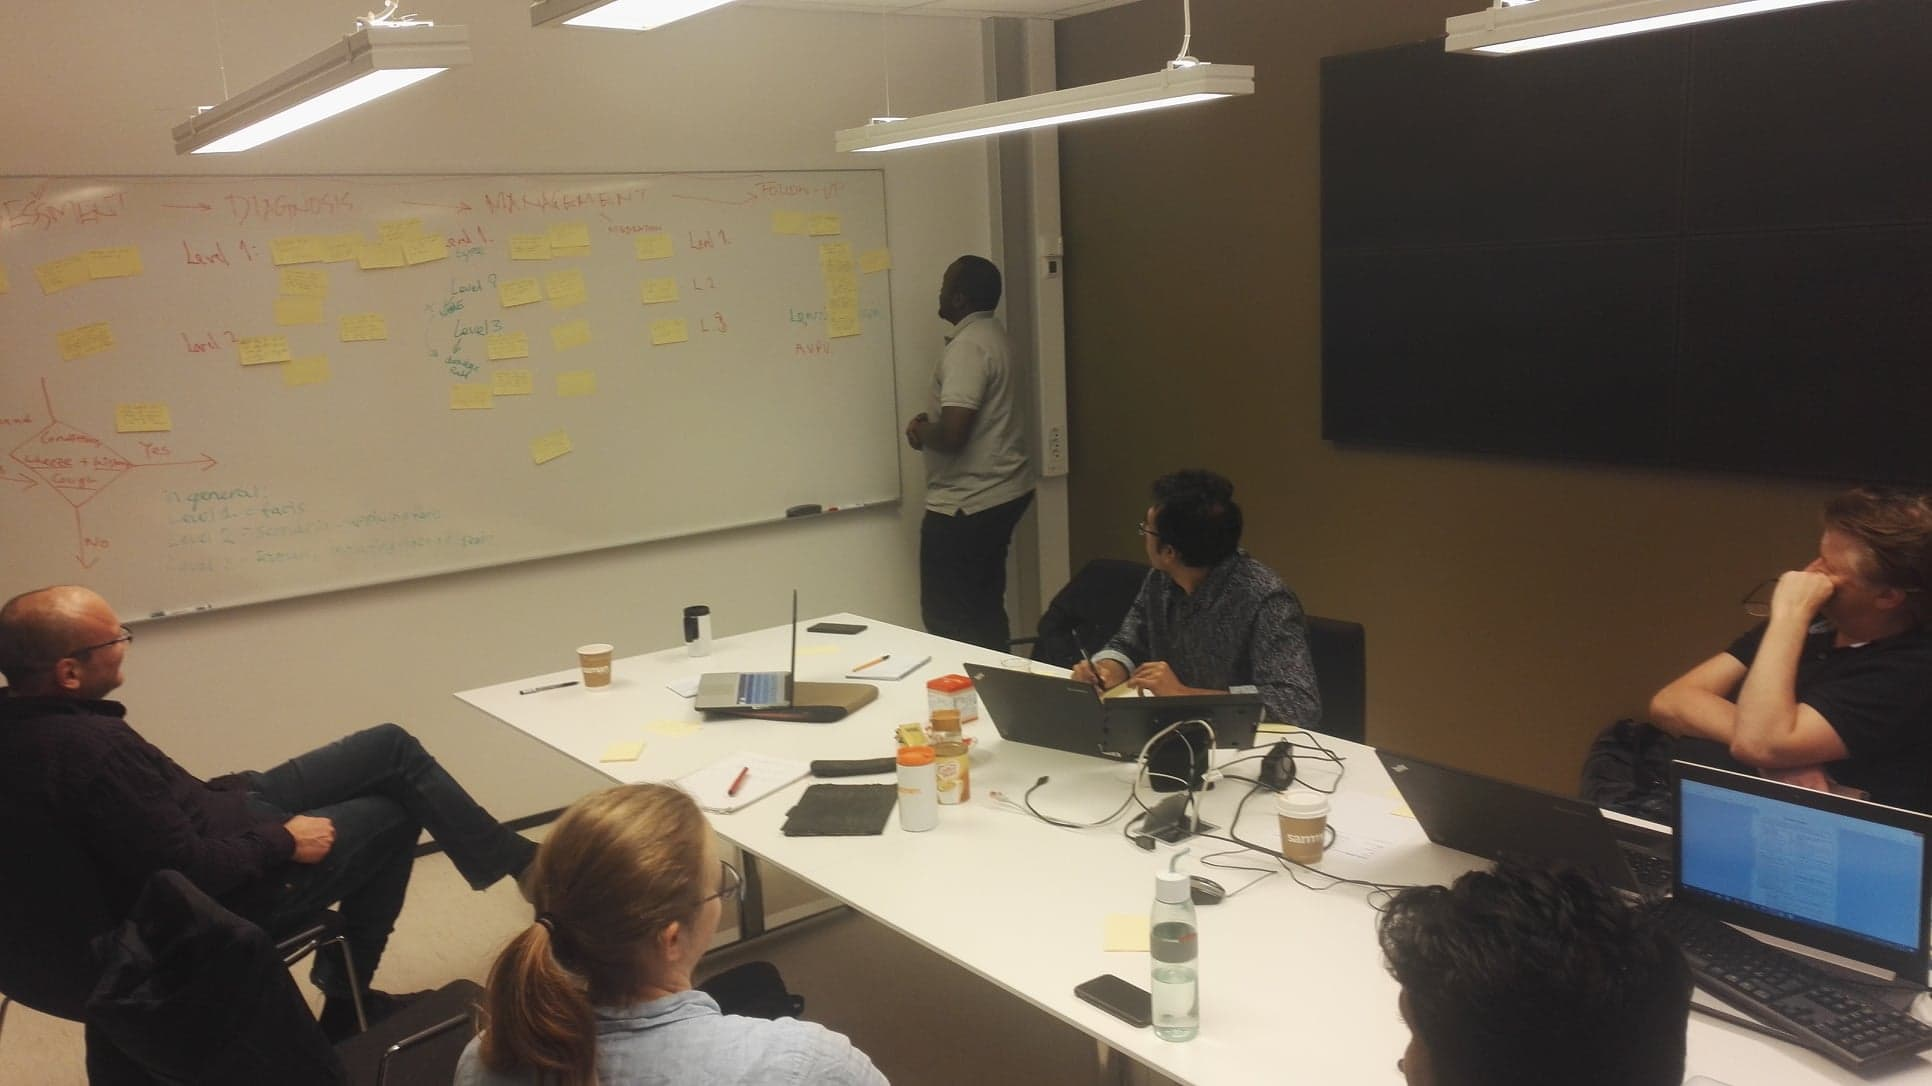
\includegraphics[scale=0.25]{workshop220219}
\end{figure}

The meeting started with Ben-Richard informing the status of the project by doing a cognitive walk-through and a demonstration of the application. 

Yngve presented ideas for further development of the application. The important thing, was the concept of splitting up the questions in themes which relates to components in the treatment plan. Job helped identify these themes as assessment, diagnosis, management and treatment. Further we identified what type of questions we wanted to ask, and how they fits into different difficulty levels, based on the details of the questions. We ask factual questions for level 1. We use scenarios in level 2, where we apply facts and the detail level is categories. I.e. what class of medication should be administered to the patient. In level 3 we continue with scenarios, but here we ask for much more details, like the dosage of a medication or how often it should be administered.

When playing level 1 the student should get questions from all themes in level 1. When the student completes level 1, the student should no longer get questions from that theme. This is to avoid boring the user by repeating the questions the student already knows the answer of. He should only get questions from themes he struggles with. I.e. on the first run level 1, the user gets every question in assessment right, but have some mistakes with diagnosis and management. Then on the next run, he only gets questions from level 1 diagnosis and management. This continues until he has reached the passing condition on every theme in level 1. 

We further identified a dependency in the treatment plan. To be able to do a follow-up, the students first needs to know something about assessment, diagnosis and management of the patient. The follow-up is actually an evaluation of the treatment which have been given, based on the suggested diagnosis. The evaluation will tell how the patient responded to the treatment, and we need the student needs to take actions whether the patient responded or his condition became better or worse. When we have such a dependency, the student needs to complete assessment, diagnosis and management before follow-up gets unlocked. Since follow-up is only relevant in a situation where there has already been set a diagnosis and given a treatment, the follow-up is only part of level 2 and 3, where the questions are given as scenarios.

To complete a level, all passing conditions at that level in each theme have to be met. When the student qualifies for a new level, he only gets questions from the level he plays. The same concept of only getting questions from the themes at that level you haven't met the passing condition, continues for level 2 and 3. 

We planned to have a visualization of the passing condition in the application. The passing condition will be shown in a chart in the summary section after each game. The passing condition will be marked as a line over every theme for the level the student plays. The students scores for each theme at that level be shown as bars. When a bar reaches the line, a passing condition is met.




\begin{figure}[h!]
	\caption {Assessment and diagnosis are components in the treatment plan. In the learning map they are themes. Under each theme there are difficulty levels. Questions for each level are written on post-it notes.}
	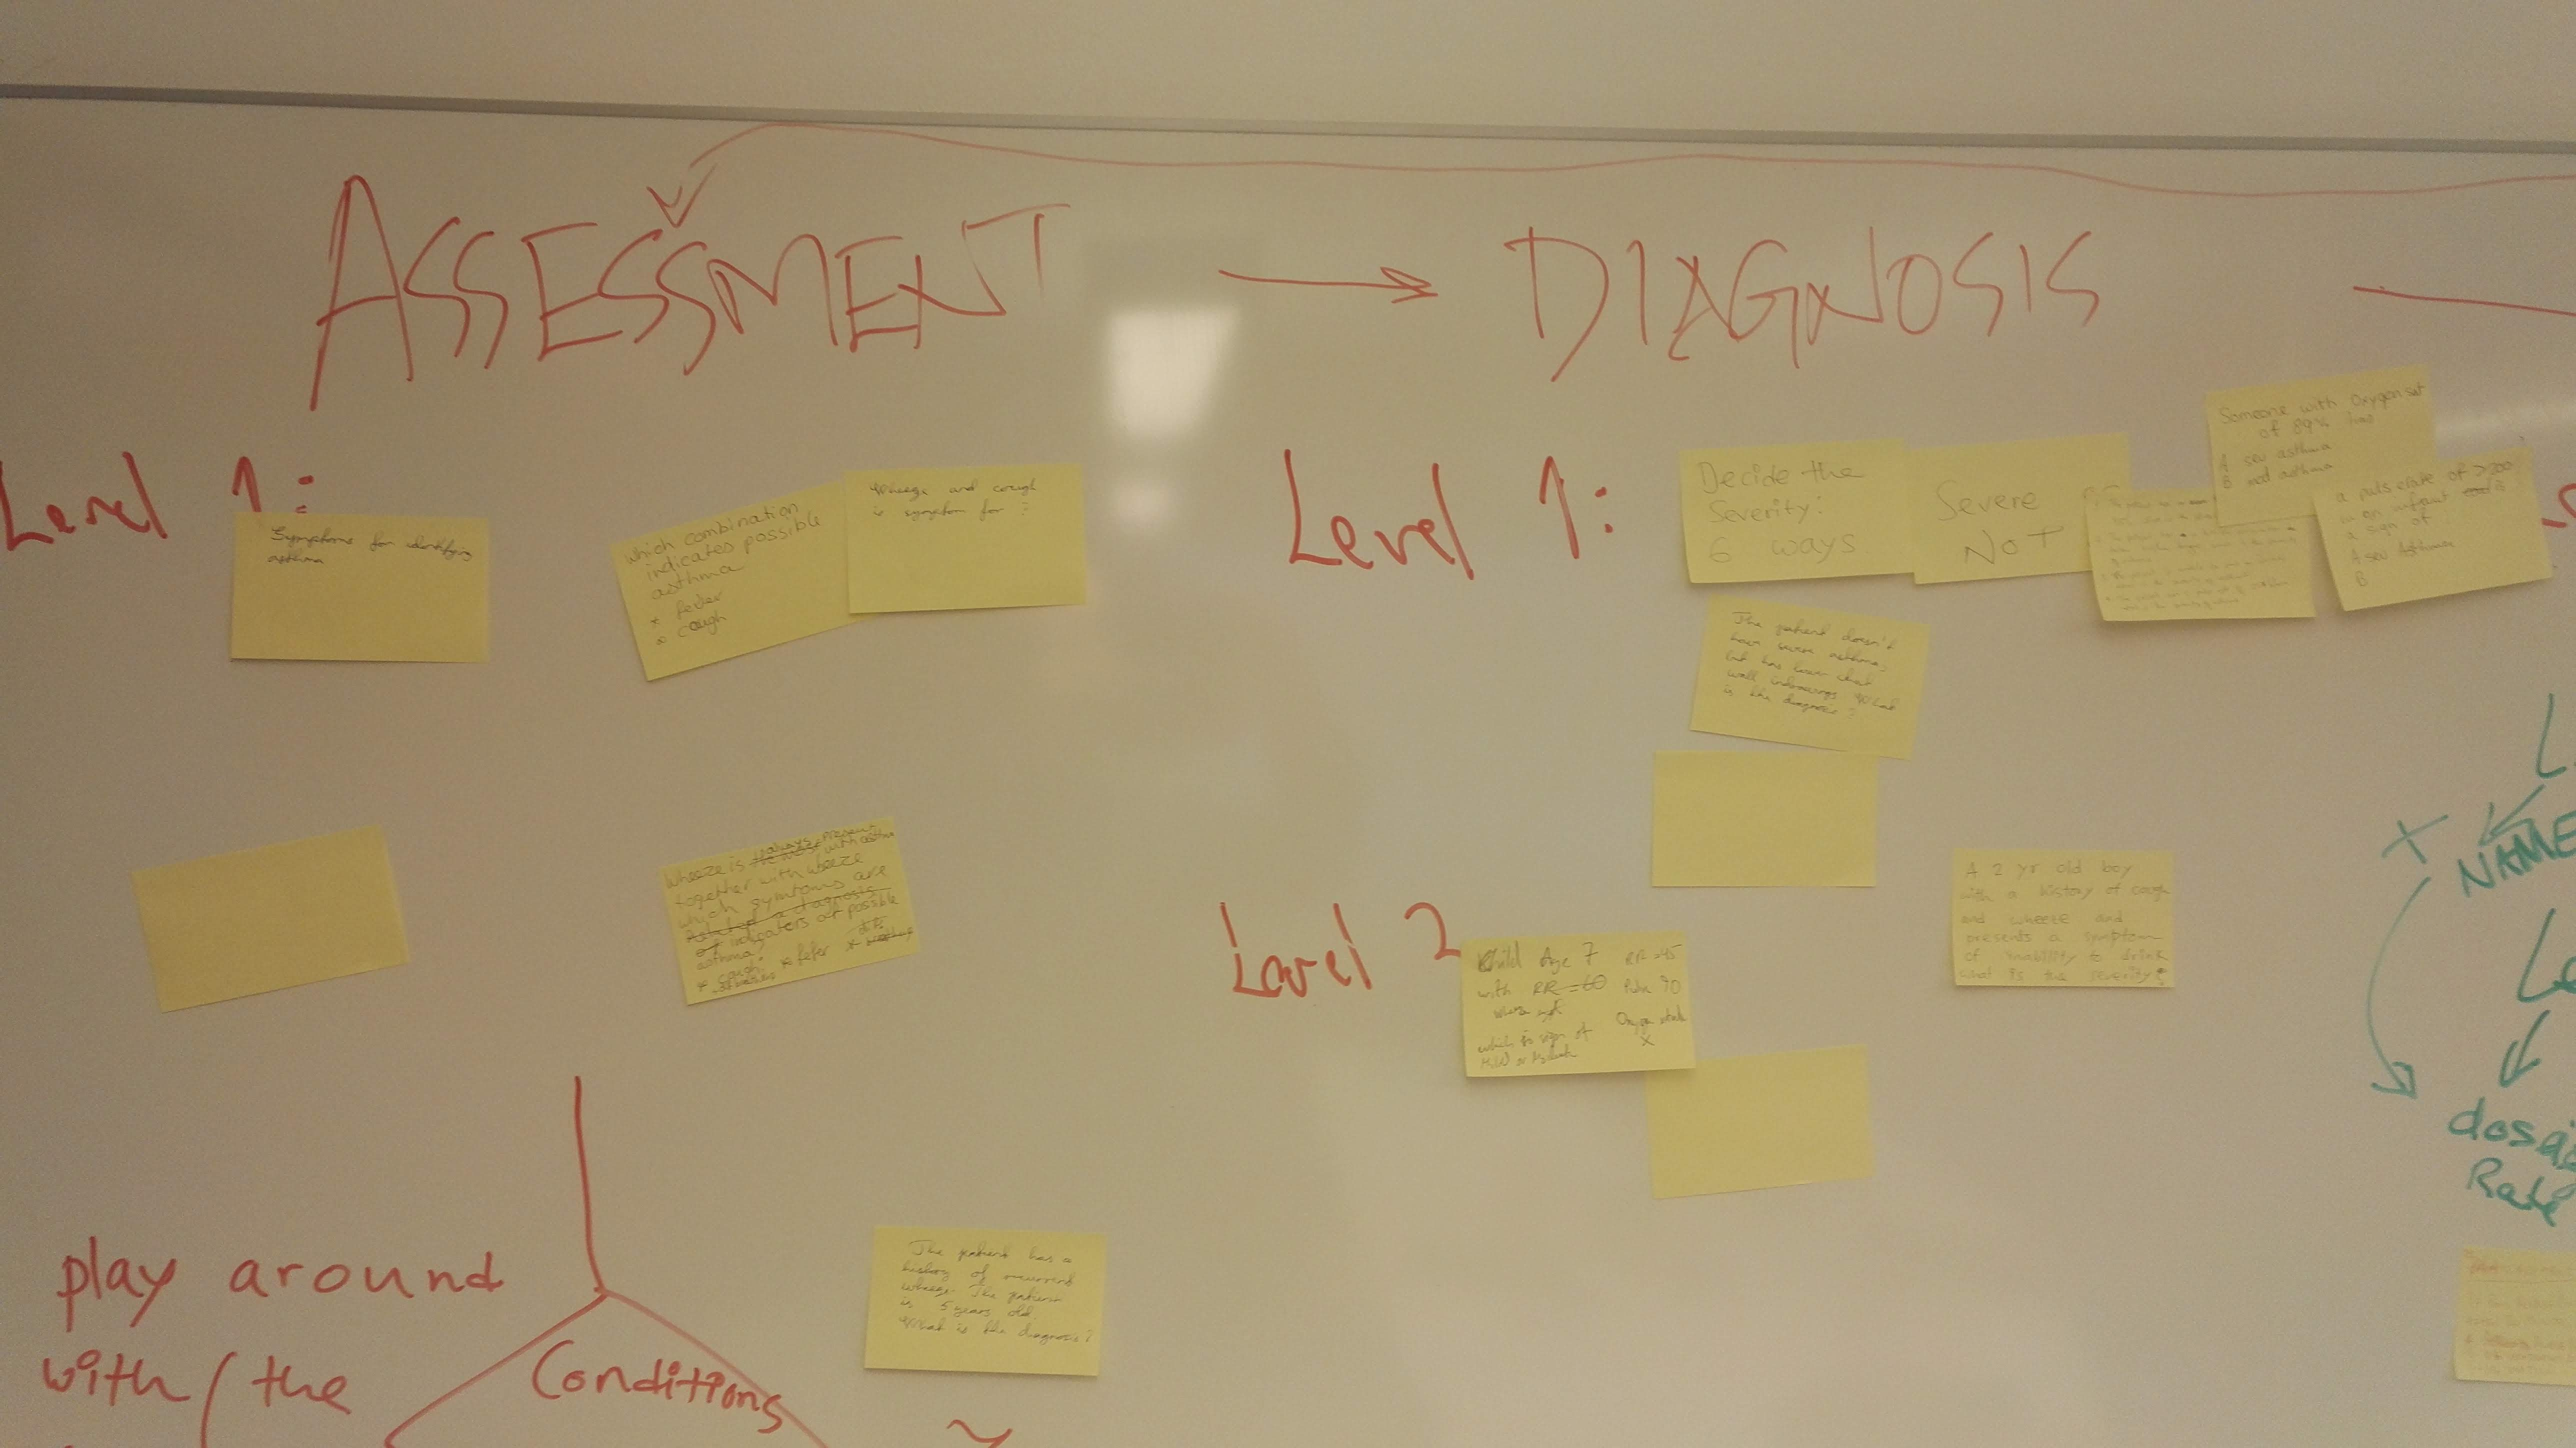
\includegraphics[scale=0.075]{workshop220219-2}
\end{figure}

\begin{figure}[h!]
	\caption {Management and follow-up are components in the treatment plan. In the learning map they are themes. Under each theme there are difficulty levels. Questions for each level are written on post-it notes.}
	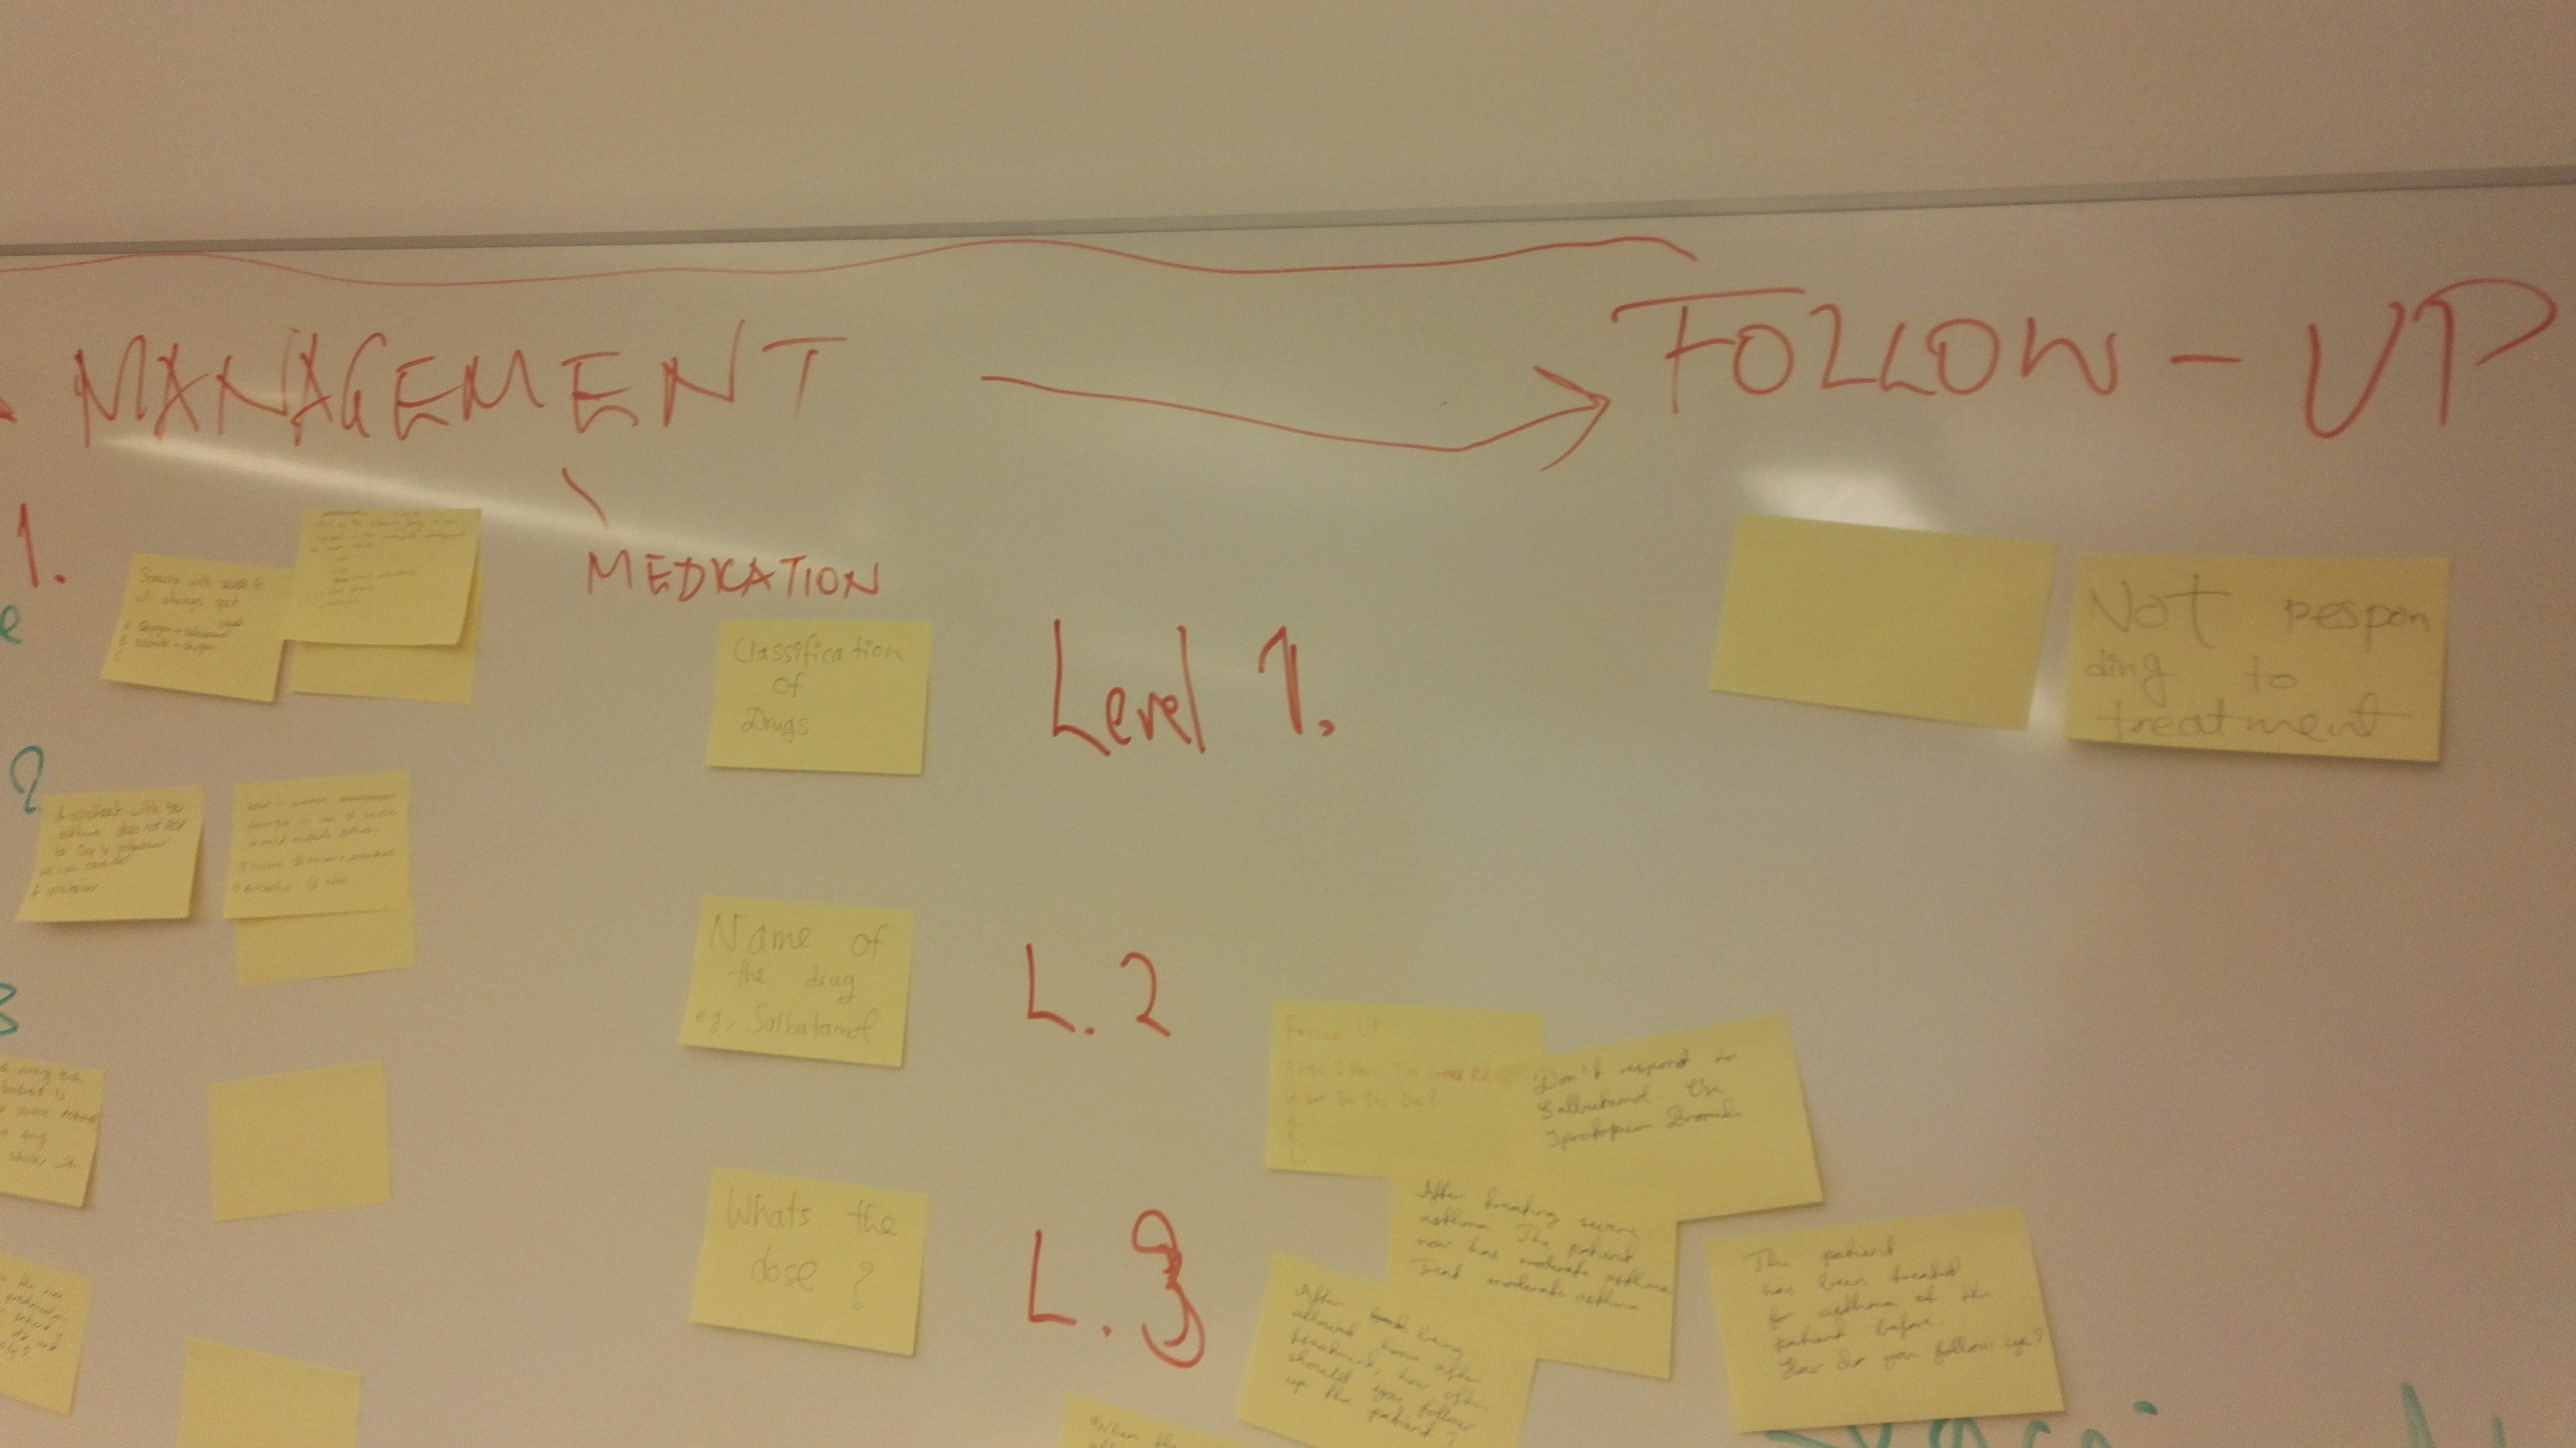
\includegraphics[scale=0.075]{workshop220219-3}
\end{figure}

\begin{figure}[h!]
	\caption {What type of questions the student will get at each level.}
	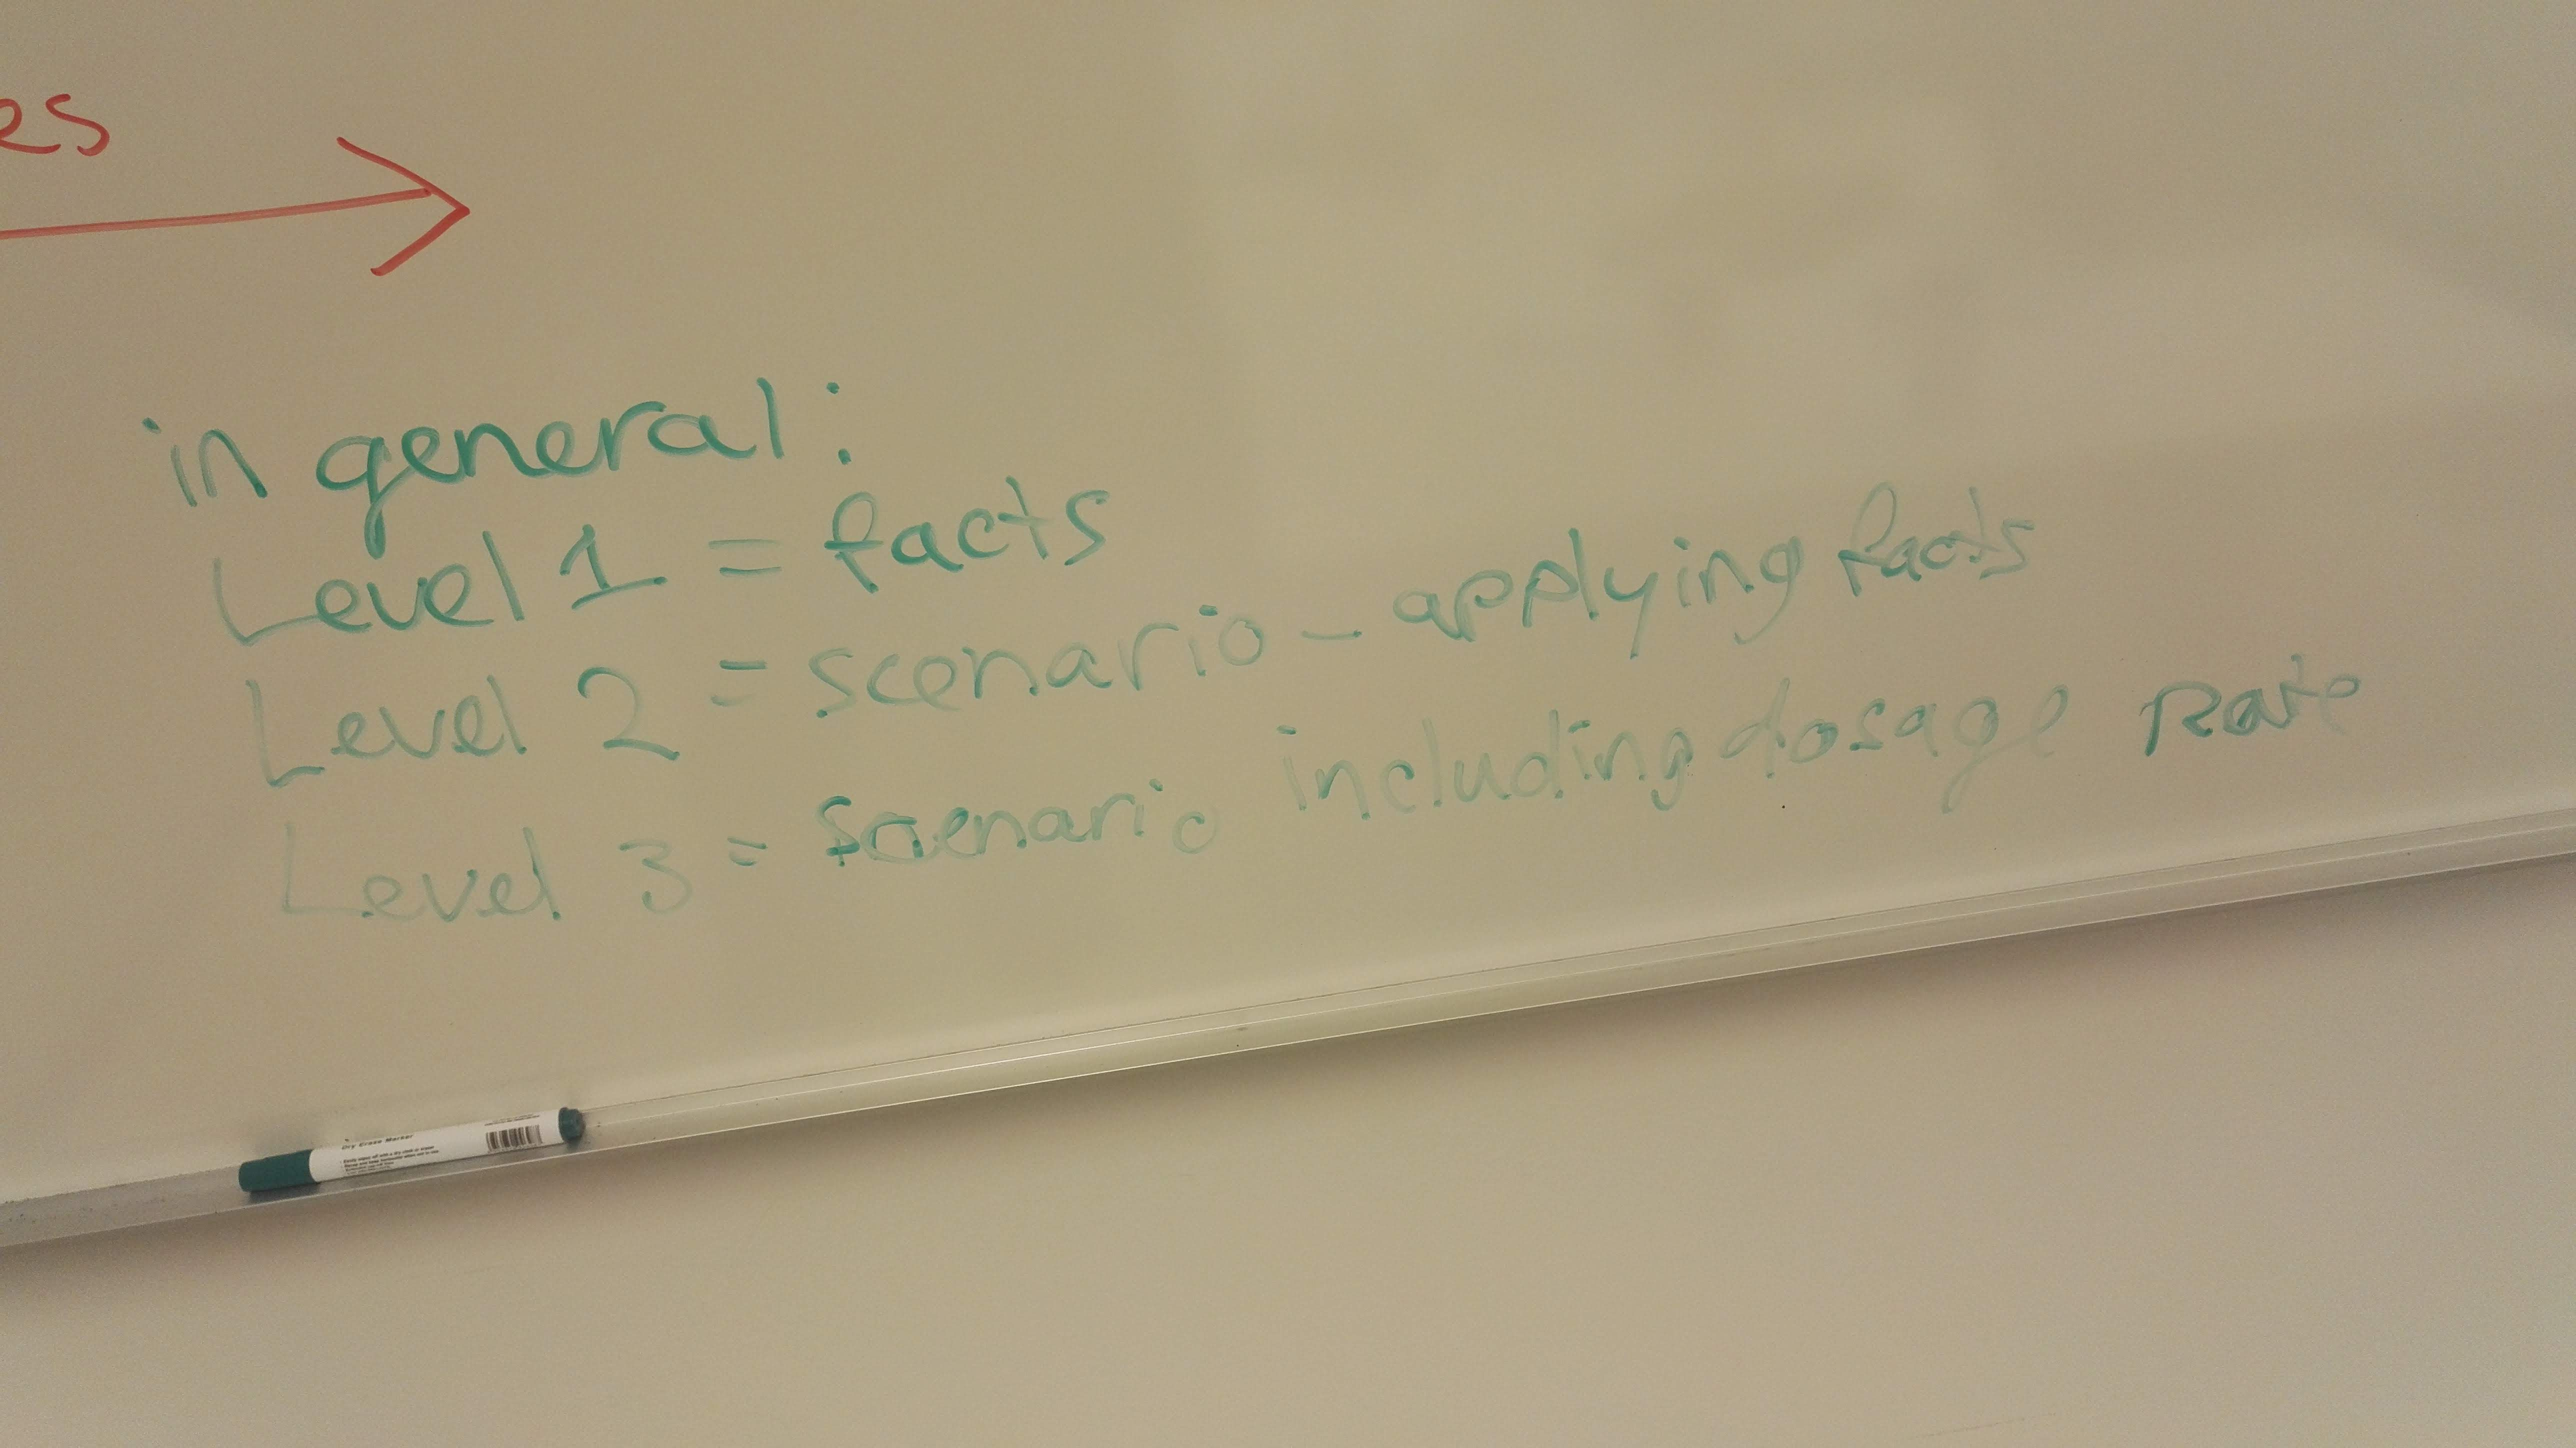
\includegraphics[scale=0.075]{workshop220219-4}
\end{figure}

Job continued the meeting by talking about the guidelines.The paediatric guideline of asthma is called "possible asthma". That is because in an emergency situation asthma is the most dangerous airway condition and can be lethal. If the patient shows signs of asthma, he will be treated for asthma to reduce risks of an unwanted scenario.

We identified users of the application: 
\begin{itemize}
	\item Formal training, where last year students are reading for their exams.
	\item Anyone can learn, so it can be used to inform and educate the public.
	\item In countries such as Kenya, where there are a large deficit in doctors and nurses, sometimes nurses has to work as doctors. Or community workers need to take the role as doctor or nurse. The application will help educating nurses and community workers for such scenarios.
\end{itemize}
 
 There was also talked about how the situation in medical training is for the student. When a patient comes to the emergency room with severe asthma, the medical doctors will have all their focus on that particular patient. The medical student will typically not take part in the assessment, diagnosis or the initial treatment of the patient. The medical student will typically only take part in the monitoring, evaluation and follow-up of the patient, when the situation is less critical. The application will give the medical student an alternative way to train in assessment, diagnosis and initial treatment of a made-up patient with severe asthma. 

Job continued the workshop by going through the Kenyan paediatric guideline of possible asthma \cite{RepublicofKeny2016}. This is the guideline we will base our quiz on. Job answered questions from the group about details of the guideline. It is important to understand the general flow as well as the details to be able to make good questions for the quiz. The guidelines is poorly written in terms of wrong use of sentential operators. These mistakes needed to be clarified.

The rest of the workshop was for the participants brainstorming around the questions which will be used in the quiz. Each participant wrote questions on post-it notes, and placed them at a suiting level and theme on the blackboard. At the end, Job went through the questions and we had a small discussion around the suggested questions. We managed to produce question templates to be used in asthma quiz of the application.

\begin{figure}[h!]
	\caption {Suggestions for questions were written on post-it notes and attached to a difficulty level under a theme on the black board.}
	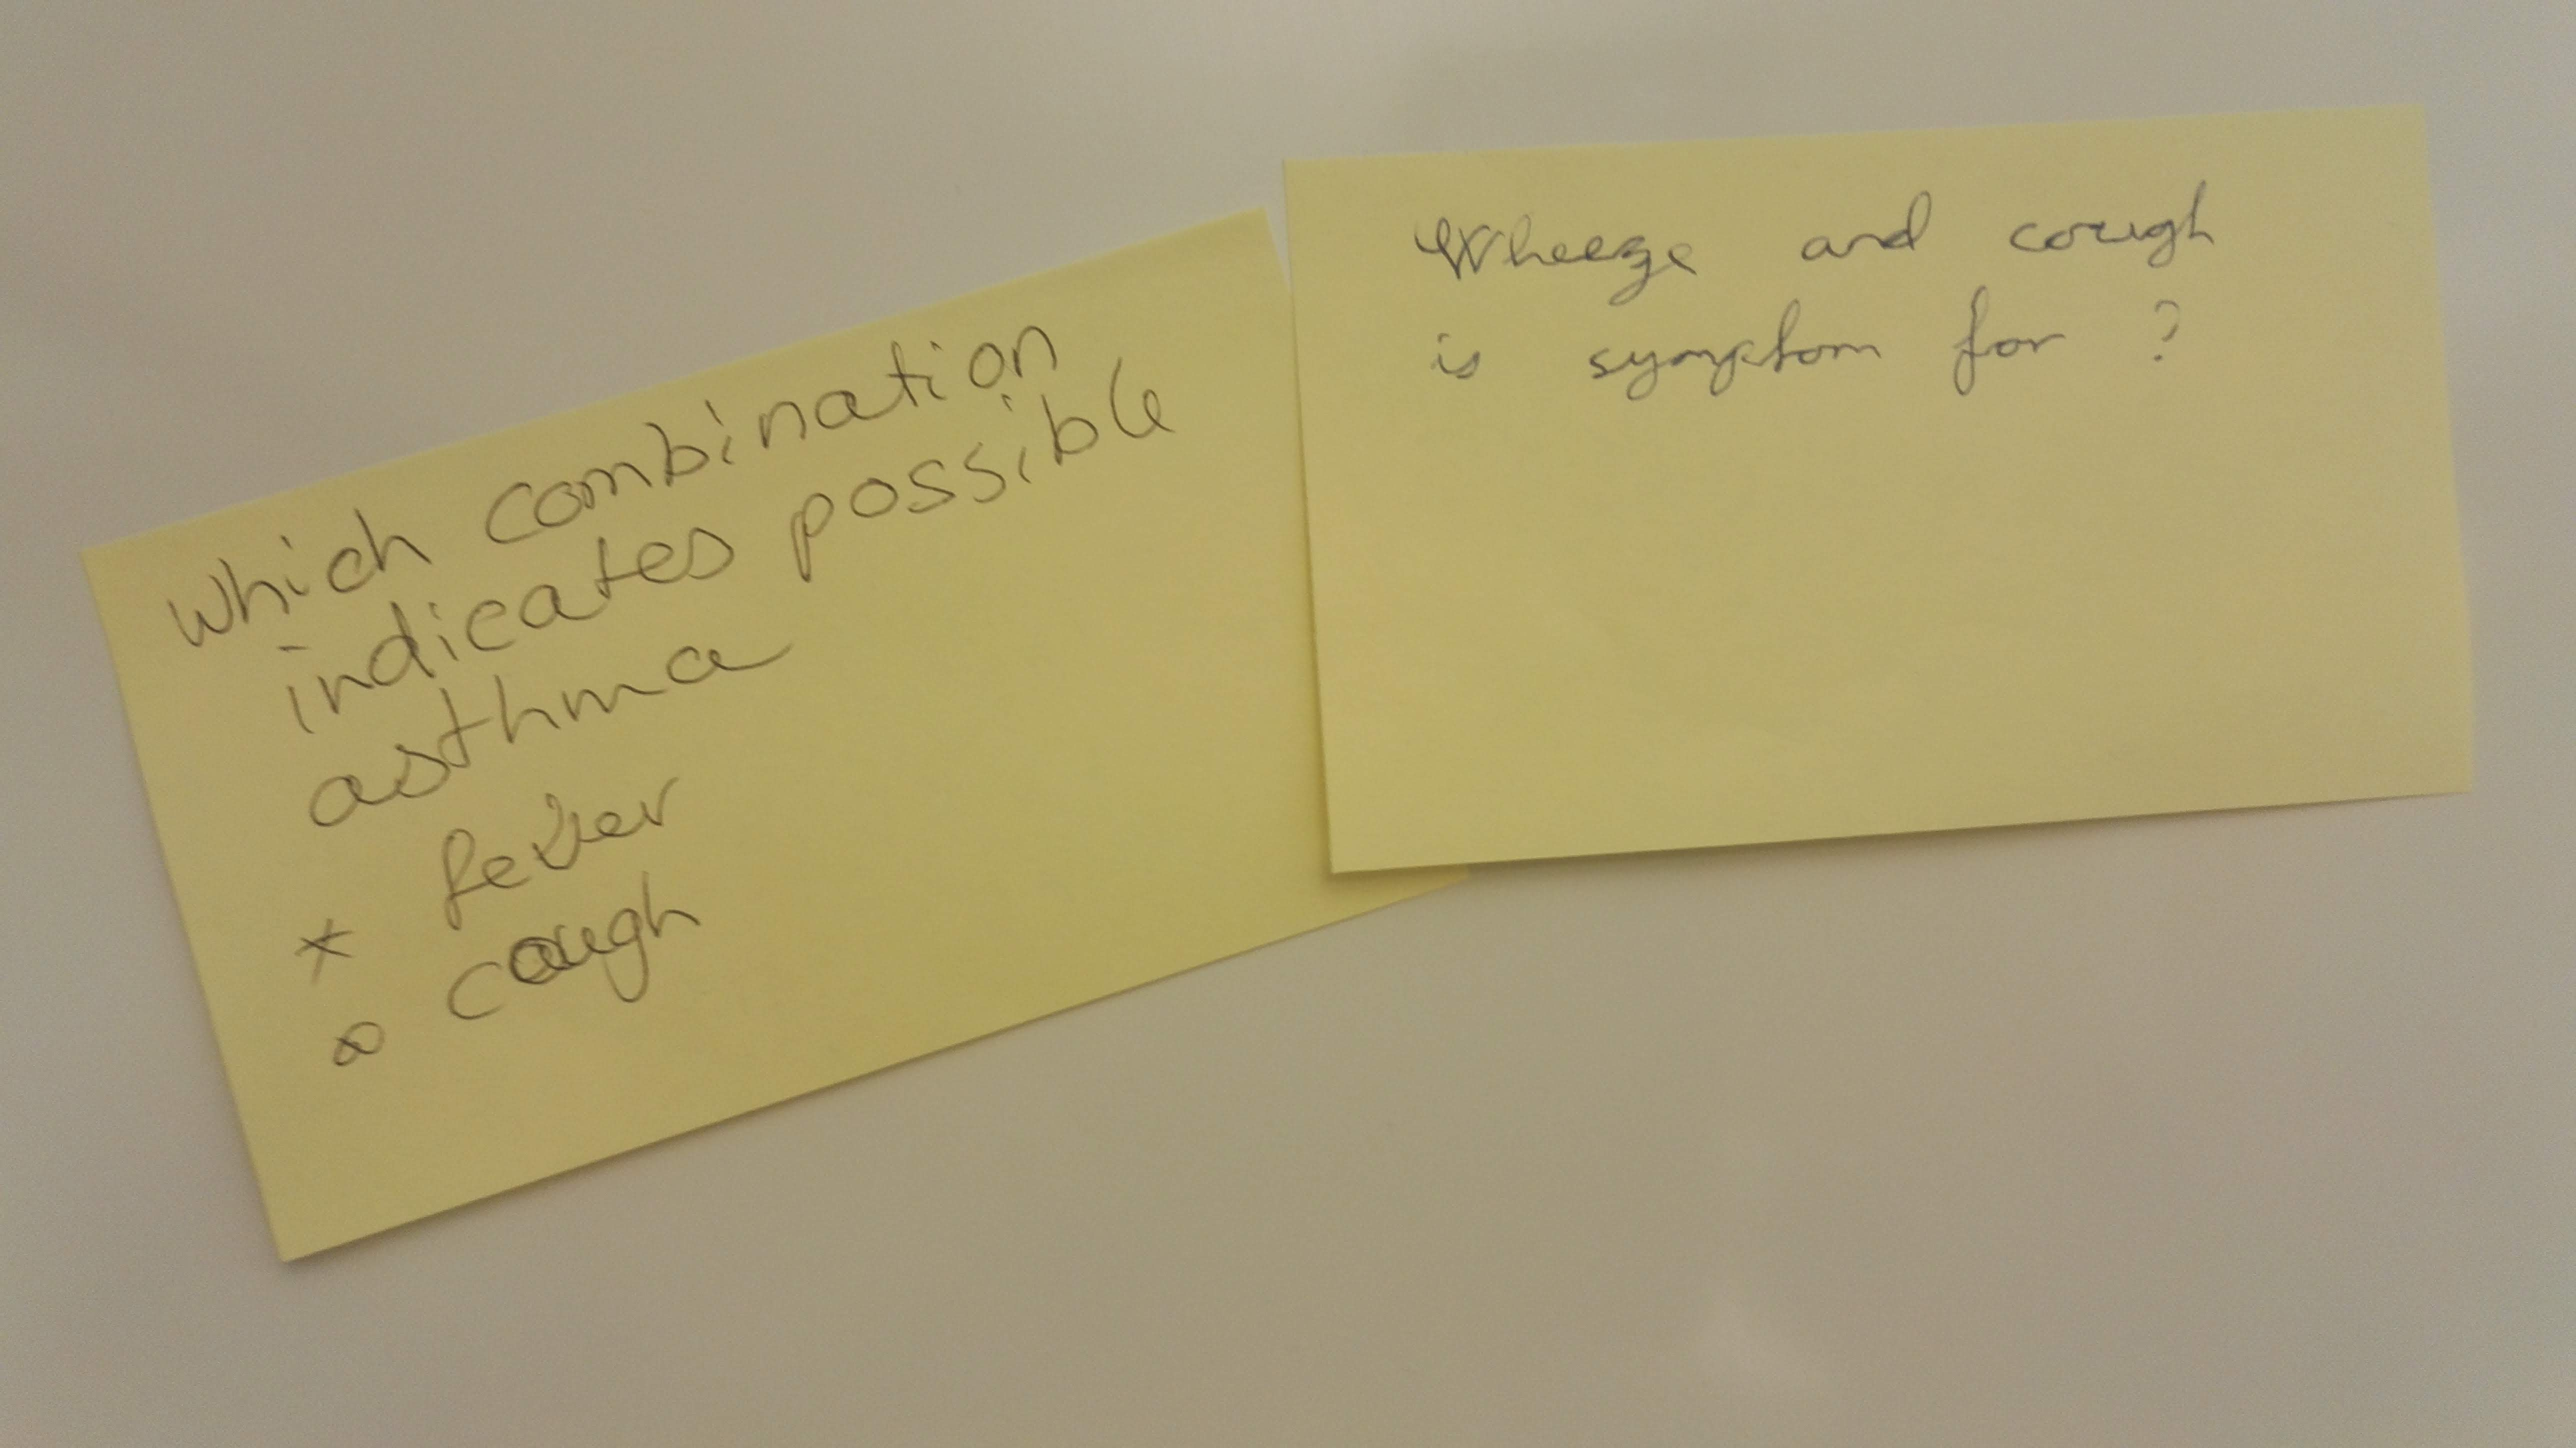
\includegraphics[scale=0.075]{workshop220219-5}
\end{figure}




\chapter{Developing a learning tool for health workers}
\section{Extracting knowledge from the clinical  practice guidelines}
\section{Data models}
\subsection{DPF metamodeling}
\subsection{Entity model}
\subsection{Workflow model}
\subsection{Game model}
\section{Game engine}
As each question in a quiz are related to a certain component in the treatment plan or theme in the learning map, the student will be measured how well he performs on each of these themes. For the asthma guideline \parencite{RepublicofKeny2016}, we have identified four themes. Assessment where the student will be tested in the initial examination. Diagnosis, where the student will determine a diagnosis as well as the severity. Management, where the student will determine which actions should be done to treat and best give the best care to the patient. The last discipline is the follow-up, where the student will be tested in evaluating the treatment, give advise to and educate patient and caregivers, provide the right medication and regular follow-up.

By splitting up the score in themes, the student can easily see which areas he is strong and where he needs more training. 



We can also adapt the questions in each discipline to the student's level. If the student has proven to be very good in providing the right amount of medicine to asthma patient, we can provide more difficult questions to challenge the student some more. If he struggles at setting the right diagnose, we can provide more basic questions to strengthen the students basic knowledge. 

\textcolor{red}{The disciplines should be automatically picked from the entity (and worflow?) model.}

\textcolor{red}{The tree structure of discipline scores. Diagnosis have examination, investigation, setting the severity. Management have advises, medication, admit, surgery and so on.}




The student will also be provided with a total score, which will be the average score of each of the disciplines. The student can compare the total score of e.g. the asthma quiz and the jaundice quiz, and see which medical condition he needs to train more on.

\subsection{Multiple-try feedback}
% https://books.google.no/books?hl=en&lr=&id=GgCPAgAAQBAJ&oi=fnd&pg=PA125&dq=Interactive+with+multiple+tries+&ots=A9Z_BJS5t2&sig=RTv1FmOzU_qic9ADjDgKdJoHamU&redir_esc=y#v=onepage&q=Interactive%20with%20multiple%20tries&f=false
% https://onlinelibrary.wiley.com/doi/full/10.1348/000709905X39134
The quiz uses a concept which is called multiple-try feedback (MTC). That means for every question the student gets more than one attempt to get the answer right. A feedback will be given immediately after each answer is submitted. The feedback consists of a message which tells whether the answer is correct or wrong. If the answer is correct, the user will receive "correct" and an explanation of the answer. If the answer is wrong, there will be no hints or explanations than just "incorrect".

\begin{tabular}{ | m{10em} | m{6em}| m{6em} | m{6em} | m{5em} | } 
	\hline
	Concept & Abbreviation & Feedback after each question & Multiple attempts at each question & Hints on wrong answer \\ [0.5ex]
	\hline
No or delayed Feedback & NF or DF & No & No & No  \\
Knowledge of Correct Response & KCR  & Yes & No & No \\
Multiple-Try feedback with knowledge of Correct response  & MTC & Yes & Yes & No \\
Multiple-Try feedback with Hints & MTH & Yes & Yes & Yes \\
\hline
\end{tabular}

The point of doing MTC, is to make the student think over what was wrong with his first answer. Did the student misinterpreter the question? Was there a detail he missed? Does the student lack the knowledge or was he just sloppy in his first attempt?

\textcite{Clariana2006} did a study where they divided 82 students into five groups. DF-, KCR, MTC and two control groups. The first control group got a text and a question at the end. The second control group got a text, but there were no question given. After 5 days,post-test was held to see what the students had learned and remembered. The post-test questions were either identical to the questions in the learning material, transposed where the order of the stem of the question and the correct-response gets reversed, paraphrased where post-test questions had the identical content as the learning material, but the phrasing was different and used different words, and a combination of transpose and paraphrasing. The results showed that DF and KCR groups performed better on identical, transposed and paraphrased-transposed questions. MTC performed better on paraphrased questions. The conclusion was that DF and KCR was much better methods for remembering the learning material word for word, but MTC was better when you have to think and reason about what you have learned.

\textcite{Attali2015} further did a did a study on NF, KCR, MTC and MTH using open ended and multiple choice questions on mathematical problems. They showed that solving an open ended question rather than multiple choice was a more efficient way to learn. The learning outcome was the same for the students using NF and KCR. However the learning transfer was greater when using multiple-try (MTC), and even more so when getting a hint on incorrect answer (MTH). They explained the results effortfull and mindful problem solving. In a multiple-try feedback, the user will have to reflect on their errors, re-evaluate the problem and understand the initial error. An open ended question will also require more effort of the student, as they have to generate a an answer rather than selecting from alternatives. On the combination of multiple-try and multiple-choice, it was suggested that some users might be less likely to review their incorrect answer and mindlessly clicking on another alternative. 



According to \textcite{Morrison1995}, students which perform badly on answer until correct questions,  will often become frustrated, loose interest for reviewing the material and probably depress learning.

% From Attali2015, students might assosiate distractions with the scenario in multiple-choice, which is counterproductive when it comes to learning.


As thinking and reasoning about a diagnosis, treatment plan, evaluation and follow-up of a treatment is part of a medical procedure, we believe that multiple-try feedback is the right approach. Because of the nature of a mobile app, where gestures are more convenient than typing sentences, multiple-choice seems to be the right choice even, though open ended questions has proven better results in. There's also a technical problem with evaluating free typed sentences.

Some of the questions in the app are too simple for a hint to be meaningful.Example: "the symptoms for asthma is" and the answer can be "cough and wheeze". Where hinting "cough", would be giving away the answer, especially in a multiple-choice format. However, the data model supports hints as links to external learning material. E.g. the student could look for the answer in the guideline itself.

We solved the "answer until correct"-problem described by \textcite{Morrison1995}, by having a "read more" button displayed upon incorrect answer. The "read more"-button will display the correct answer, an explanation and continue to the next question. Avoiding the user becoming frustrated and discouraged by having to brute-force the answer keys to progress.




\subsection{Reward system}
% SHOW ANSWER
By having multiple-try feedback, another problem rises, and that is the reward system. If there is no penalty for incorrect answers, a student which needs ten attempts per questions, will get the same score as a student which answers all the questions correctly on the first attempt.

\textcite{Attali2015} solved the problem by giving 1 point for answering correctly on the first attempt. 2/3 points for the second attempt, 1/3 for the third and 0 points if the third attempt was incorrect. A limitation with this method is that it makes no sense for the student to make more than three attempts. \textcite{Morrison1995} had another strategy where they adjust the scores by dividing the total score by the total number of attempts during the quiz. A consequence is that attempt number two will have a huge penalty which is halving the students total score. While attempt number twenty will give a very small penalty from attempt nineteen.

The solution we used was having a fixed value for every answer alternative. The quiz author chooses the penalty for each distraction and reward for each answer key. The idea is that the distractions can have some sort of degree of wrong or right, and this can be reflected in the scoring. On the question "what are the symptoms of asthma?", "difficulty breathing" is a more correct answer than "fever", as "difficulty breathing" is a symptom of asthma in combination with wheeze. Fever is not an asthma symptom at all. In future work, the penalties can be automated as you can see from the entity model whether the symptom belongs to the asthma guideline or not. A distraction from respiratory disorders may give a larger penalty than a distraction from the asthma guideline, but smaller penalty than symptoms not belonging to respiratory diseases.

Both \textcite{Attali2015} and \textcite{Morrison1995} avoids the scenario where the user gets a total minus score. This may be a strength of these methods, as a negative total score seems like a very harsh feedback and might demotivate the student. In our solution we use negative numbers as penalties on distractions, such that a negative total score may happen. We try to limit the likelihood of a negative score by providing a very reward for a correct answer and a very small penalty for a distraction. Typically the reward is 10 points and the penalty -1 og -2 points. The intention is to encourage the student to review the incorrect answer and try again. As the format is multiple-choice and the penalty-reward ratio, there is a little risk involved trying multiple times. But giving up by clicking "learn more", the student will not get an additional penalty, but will miss out on the reward. By clicking answer alternatives mindlessly and consequently clicking "learn more" will probably not end up in a negative score, but is more likely to end up in a negative score than mindlessly click answer alternatives until correct.

%----------------------------------------------------------------------------------


%Each question will have several answer alternatives the student can choose from. Each answer alternative will have a reward or penalty related to them. The correct answer will have a great reward, while wrong answers will have a small penalty. The quiz author will have the opportunity to specify the rewards, such that he can give even smaller penalties for partly correct answers. The idea of the reward- penalty system is to increase learning. if the student answers wrong the first time, he will be given the possibility to reflect over the question once more or perhaps read the guideline to learn before he commits his second attempt. We are aware that providing a minus score for making an attempt can be very demotivating, but it is to avoid the situation where a student gets the same (or better) score for making ten attempts than only needing one attempt. A small penalty will have a very small impact when the reward per question is high, but in situations where the student performs very poorly and ends with a negative total score, it is possible to adjust this to a small positive score on presentation for the student. Not giving a too harsh feedback for trying to learn.



\textcolor{red}{A solution to having a not very strict game, encouraging to playing and learning, one can also have a very strict examination version. The idea is that after examination, the results will be sent to the lecturer (or a governing body of some kind) to evaluate what the overall knowledge of the students, as well as details of what the students are really good in and where do they struggle. The lecturer can then target the weak of points of the students in one of the next lectures. }


\subsection{Unlocking harder levels at a certain category}
\textcolor{red}{(somewhere in the paper I need to refer to Eides, Kristensens and Lamos paper, and discuss the knowledge, learning and student maps and that they need to prove basic knowledge in some disciplines before they can unlock content in other disciplines.)}
\subsection{Visualization of game statistics}
\subsection{Automatically generating new questions}
\section{The mobile application}
\begin{itemize}
	\item React
	\item React-Native
	\item React-Native-Navigation (Wix)
	\item Redux
	\item React-Redux
	\item Redux-Thunk
	\item Highcharts
	\item Jest
\end{itemize}
\subsection{React-Native and Redux}
\subsection{User interface and flow of the user interaction}
\section{Architecture of the whole system}
\subsection{Visualization}
\section{Evaluation}



\chapter{Discussion}
\section{Research questions}
\section{Limitations of the model}
\begin{itemize}
	\item Can't ask questions like "what are the symptoms for severe asthma?"
	\item Difficult to ask what NOT to do. If the vertex doesn't exist, only an empty string gets returned. Can only be used were we actually have written "don't admit to the hospital" as an example with hospitalization.
	\item The inheritance makes it difficult to generalize some questions. We can't make a template which asks about the Rate a medicine should be taken with. We need to specifically ask for that medicine. To be able to ask for a general medicine, one solution can be to introduce a new tag which compares the substring of the type of the vertex. Another solution is to use the meta model and not the instance model. We don't use inheritance on diagnosis because of this.
	\item To avoid the problem described in the previous point, we don't use inheritance on Diagnosis. A limitation here is that  
	a patient can only have one diagnosis.
\end{itemize}
\section{Observations}
\section{Challenges}
\section{Reflection}



\chapter{Conclusions}
\section{Further research and development}


\backmatter
% bibliography, glossary and index would go here.
\end{document}